% Options for packages loaded elsewhere
% Options for packages loaded elsewhere
\PassOptionsToPackage{unicode}{hyperref}
\PassOptionsToPackage{hyphens}{url}
\PassOptionsToPackage{dvipsnames,svgnames,x11names}{xcolor}
%
\documentclass[
  letterpaper,
  DIV=11,
  numbers=noendperiod]{scrartcl}
\usepackage{xcolor}
\usepackage{amsmath,amssymb}
\setcounter{secnumdepth}{-\maxdimen} % remove section numbering
\usepackage{iftex}
\ifPDFTeX
  \usepackage[T1]{fontenc}
  \usepackage[utf8]{inputenc}
  \usepackage{textcomp} % provide euro and other symbols
\else % if luatex or xetex
  \usepackage{unicode-math} % this also loads fontspec
  \defaultfontfeatures{Scale=MatchLowercase}
  \defaultfontfeatures[\rmfamily]{Ligatures=TeX,Scale=1}
\fi
\usepackage{lmodern}
\ifPDFTeX\else
  % xetex/luatex font selection
\fi
% Use upquote if available, for straight quotes in verbatim environments
\IfFileExists{upquote.sty}{\usepackage{upquote}}{}
\IfFileExists{microtype.sty}{% use microtype if available
  \usepackage[]{microtype}
  \UseMicrotypeSet[protrusion]{basicmath} % disable protrusion for tt fonts
}{}
\makeatletter
\@ifundefined{KOMAClassName}{% if non-KOMA class
  \IfFileExists{parskip.sty}{%
    \usepackage{parskip}
  }{% else
    \setlength{\parindent}{0pt}
    \setlength{\parskip}{6pt plus 2pt minus 1pt}}
}{% if KOMA class
  \KOMAoptions{parskip=half}}
\makeatother
% Make \paragraph and \subparagraph free-standing
\makeatletter
\ifx\paragraph\undefined\else
  \let\oldparagraph\paragraph
  \renewcommand{\paragraph}{
    \@ifstar
      \xxxParagraphStar
      \xxxParagraphNoStar
  }
  \newcommand{\xxxParagraphStar}[1]{\oldparagraph*{#1}\mbox{}}
  \newcommand{\xxxParagraphNoStar}[1]{\oldparagraph{#1}\mbox{}}
\fi
\ifx\subparagraph\undefined\else
  \let\oldsubparagraph\subparagraph
  \renewcommand{\subparagraph}{
    \@ifstar
      \xxxSubParagraphStar
      \xxxSubParagraphNoStar
  }
  \newcommand{\xxxSubParagraphStar}[1]{\oldsubparagraph*{#1}\mbox{}}
  \newcommand{\xxxSubParagraphNoStar}[1]{\oldsubparagraph{#1}\mbox{}}
\fi
\makeatother


\usepackage{longtable,booktabs,array}
\newcounter{none} % for unnumbered tables
\usepackage{calc} % for calculating minipage widths
% Correct order of tables after \paragraph or \subparagraph
\usepackage{etoolbox}
\makeatletter
\patchcmd\longtable{\par}{\if@noskipsec\mbox{}\fi\par}{}{}
\makeatother
% Allow footnotes in longtable head/foot
\IfFileExists{footnotehyper.sty}{\usepackage{footnotehyper}}{\usepackage{footnote}}
\makesavenoteenv{longtable}
\usepackage{graphicx}
\makeatletter
\newsavebox\pandoc@box
\newcommand*\pandocbounded[1]{% scales image to fit in text height/width
  \sbox\pandoc@box{#1}%
  \Gscale@div\@tempa{\textheight}{\dimexpr\ht\pandoc@box+\dp\pandoc@box\relax}%
  \Gscale@div\@tempb{\linewidth}{\wd\pandoc@box}%
  \ifdim\@tempb\p@<\@tempa\p@\let\@tempa\@tempb\fi% select the smaller of both
  \ifdim\@tempa\p@<\p@\scalebox{\@tempa}{\usebox\pandoc@box}%
  \else\usebox{\pandoc@box}%
  \fi%
}
% Set default figure placement to htbp
\def\fps@figure{htbp}
\makeatother

\ifLuaTeX
  \usepackage{luacolor}
  \usepackage[soul]{lua-ul}
\else
  \usepackage{soul}
\fi




\setlength{\emergencystretch}{3em} % prevent overfull lines

\providecommand{\tightlist}{%
  \setlength{\itemsep}{0pt}\setlength{\parskip}{0pt}}



 


\KOMAoption{captions}{tableheading}
\makeatletter
\@ifpackageloaded{caption}{}{\usepackage{caption}}
\AtBeginDocument{%
\ifdefined\contentsname
  \renewcommand*\contentsname{Table of contents}
\else
  \newcommand\contentsname{Table of contents}
\fi
\ifdefined\listfigurename
  \renewcommand*\listfigurename{List of Figures}
\else
  \newcommand\listfigurename{List of Figures}
\fi
\ifdefined\listtablename
  \renewcommand*\listtablename{List of Tables}
\else
  \newcommand\listtablename{List of Tables}
\fi
\ifdefined\figurename
  \renewcommand*\figurename{Figure}
\else
  \newcommand\figurename{Figure}
\fi
\ifdefined\tablename
  \renewcommand*\tablename{Table}
\else
  \newcommand\tablename{Table}
\fi
}
\@ifpackageloaded{float}{}{\usepackage{float}}
\floatstyle{ruled}
\@ifundefined{c@chapter}{\newfloat{codelisting}{h}{lop}}{\newfloat{codelisting}{h}{lop}[chapter]}
\floatname{codelisting}{Listing}
\newcommand*\listoflistings{\listof{codelisting}{List of Listings}}
\makeatother
\makeatletter
\makeatother
\makeatletter
\@ifpackageloaded{caption}{}{\usepackage{caption}}
\@ifpackageloaded{subcaption}{}{\usepackage{subcaption}}
\makeatother
\usepackage{bookmark}
\IfFileExists{xurl.sty}{\usepackage{xurl}}{} % add URL line breaks if available
\urlstyle{same}
\hypersetup{
  colorlinks=true,
  linkcolor={blue},
  filecolor={Maroon},
  citecolor={Blue},
  urlcolor={Blue},
  pdfcreator={LaTeX via pandoc}}


\author{}
\date{}
\begin{document}


\subsection{}\label{section}


\includegraphics[width=\linewidth,height=0.83333in,keepaspectratio]{../assets/images/gup-logo-transparent.png}

\subsubsection{Dramatische
Leistungssteigerung}\label{dramatische-leistungssteigerung}

\subsubsection{für produzierende
Unternehmen}\label{fuxfcr-produzierende-unternehmen}

Ehrlich. Direkt. Wirksam.

\pandocbounded{
\includegraphics[keepaspectratio]{../assets/images/icons/wertschoepfung.png}}

\subsection{Wertschöpfung \&
Wettbewerbsfähigkeit}\label{wertschuxf6pfung-wettbewerbsfuxe4higkeit}

50\%

Lieferzeiten halbieren. Ressourcen halbieren. Innovationen verdoppeln.

. . .

Kostendenken wird den typischen Mittelständler nicht retten.\\
\textbf{Höchstleistung schon.}

. . .

Schnelle Erprobung \textbar{} \st{statt sauteure Konzepte} \textbar{}\\
Echte Probleme lösen \textbar{} \st{statt Methodik bis der Arzt kommt}
\textbar{}\\
Mehr Wirkung \textbar{} \st{statt mehr Manntage} \textbar{}

\subsection{Drei Hebel für
Höchstleistung}\label{drei-hebel-fuxfcr-huxf6chstleistung}

\pandocbounded{
\includegraphics[keepaspectratio]{../assets/images/icons/image-13.png}}

\subsubsection{01 Organisation, Führung \&
Können}\label{organisation-fuxfchrung-kuxf6nnen}

Organisationen erzeugen Verhalten -- nicht umgekehrt. Wir arbeiten am
System. Da Führung das System jeden Tag wieder erzeugt, arbeiten wir an
Führung.

Führung als Gestaltungs-Kompetenz.

\pandocbounded{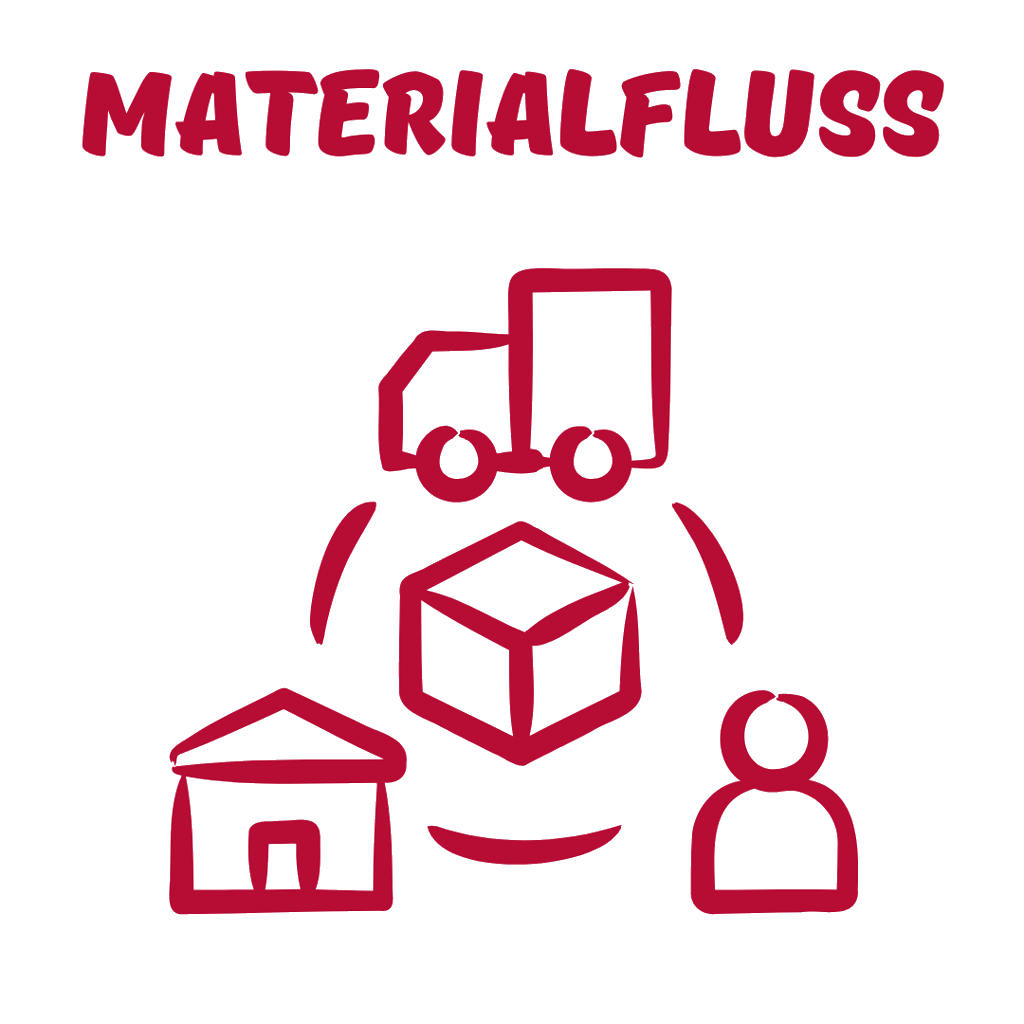
\includegraphics[keepaspectratio]{../assets/images/icons/image-09.png}}

\subsubsection{02 Lean -- also ReaLean}\label{lean-also-realean}

Ohne saugute Wertschöpfung ist alles andere nichts. Fluss erzeugen,
Engpässe lösen, Verschwendung eliminieren.

Lean ohne Methodik -- aber mit konkreter Wirkung.

\pandocbounded{
\includegraphics[keepaspectratio]{../assets/images/icons/image-12.png}}

\subsubsection{03 ERP \& KI}\label{erp-ki}

Das ERP muss Rückenwind werden, nicht Hürdenlauf. KI bringt nur etwas,
wenn Wertschöpfung wirklich besser wird.

ERP als Leistungs-Bremse -- oder Rückenwind?

\subsection{Team: Kompetenzen, die
wirken}\label{team-kompetenzen-die-wirken}

\pandocbounded{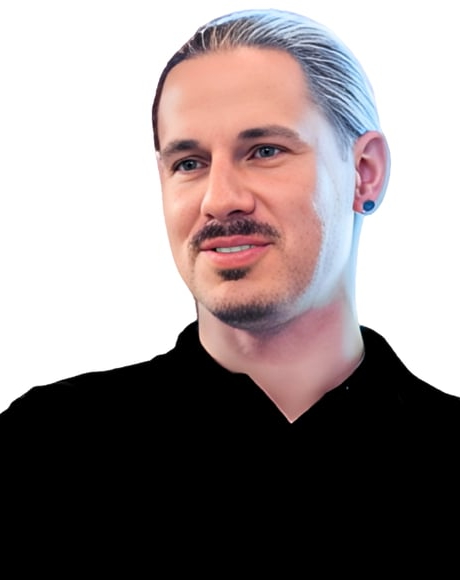
\includegraphics[keepaspectratio]{../assets/images/team/florian-final.png}}

\textbf{Florian Glöbl}\\
Geschäftsführer, Berater \& Vernetzer

15+ Jahre Sondermaschinenbau

\pandocbounded{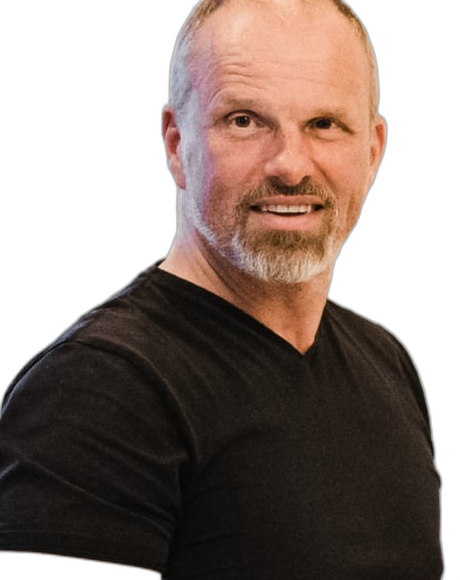
\includegraphics[keepaspectratio]{../assets/images/team/benno-final.png}}

\textbf{Benno Löffler}\\
Gesellschafter \& Systempraktiker

25+ Jahre Beratung. Autor „Saugute Zusammenarbeit''

\pandocbounded{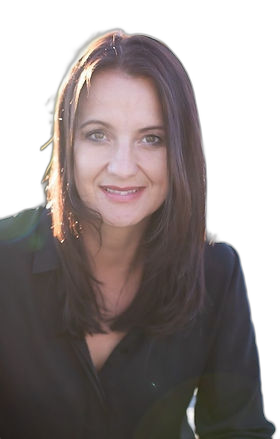
\includegraphics[keepaspectratio]{../assets/images/team/simone-final.png}}

\textbf{Simone Heigl}\\
Trainerin, Beraterin \& Coach

Kommunikation, Resilienz, Klartext

\pandocbounded{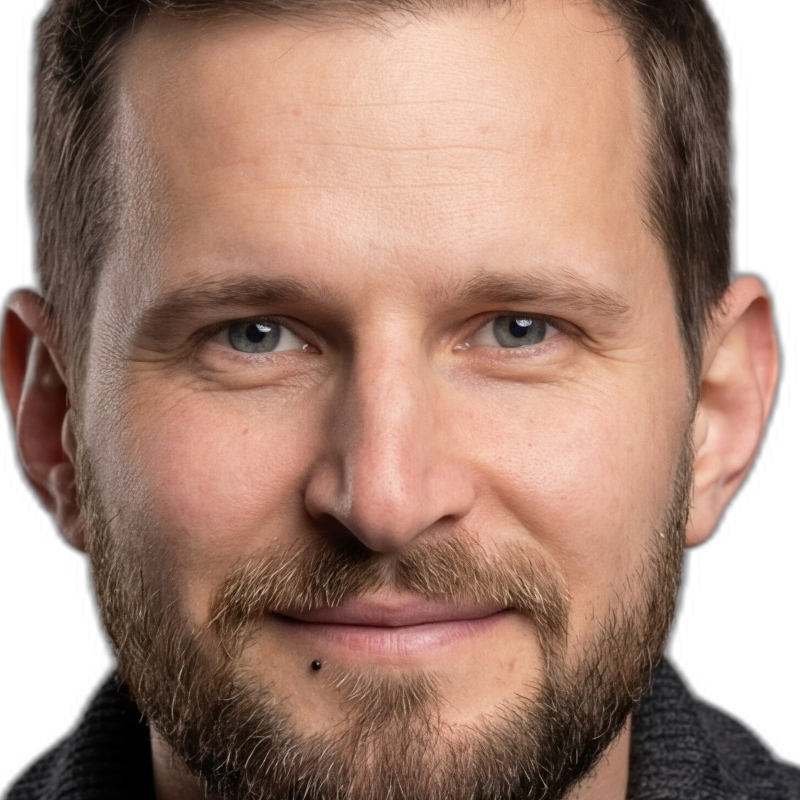
\includegraphics[keepaspectratio]{../assets/images/team/david-final.png}}

\textbf{David Weber}\\
Lean-Berater \& Wertschöpfungsexperte

Fluss erzeugen, Engpässe lösen

\subsection{Vorgehen: Das Trafo-Modell}\label{vorgehen-das-trafo-modell}

\textbf{1. Orientierung}\\
Verstehen, wo es weh tut. Klarheit über Engpässe und
Höchstleistungskiller.

→

\textbf{2. Schnelle Erprobung}\\
Kleine Experimente in der Wertschöpfung. Wirkt es? Dann mehr davon.

→

\textbf{3. Verankerung}\\
Neue Praktiken in den Alltag überführen. Führung sichert den neuen
Standard.

. . .

\textbf{Kein Riesenprojekt.} Kein Change-Management-Theater.\\
Stattdessen: Erprobung → Wirkung → Entscheidung → nächster Schritt.

\subsection{Bereit für
Höchstleistung?}\label{bereit-fuxfcr-huxf6chstleistung}

Ein Gespräch. Du erzählst. Wir stellen Fragen. Du denkst nach.\\
Und wenn Du dann nochmal sprechen willst, hat das Gespräch offenbar
etwas bewirkt\ldots{}

\textbf{Florian Glöbl}\\
f.gloebl@g-und-p.de\\
+49 (0) 172 / 1718875

G\&P Management Consultants UG\\
Birkenweg 6, 84082 Laberweinting

Gespräch vereinbaren. Klartext. Versprochen.




\end{document}
